\begin{question}
\noindent A research station stores space-mission samples in a cuboid-shaped storage box, $ABCDEFGH$, as shown in the diagram below.

\begin{center}
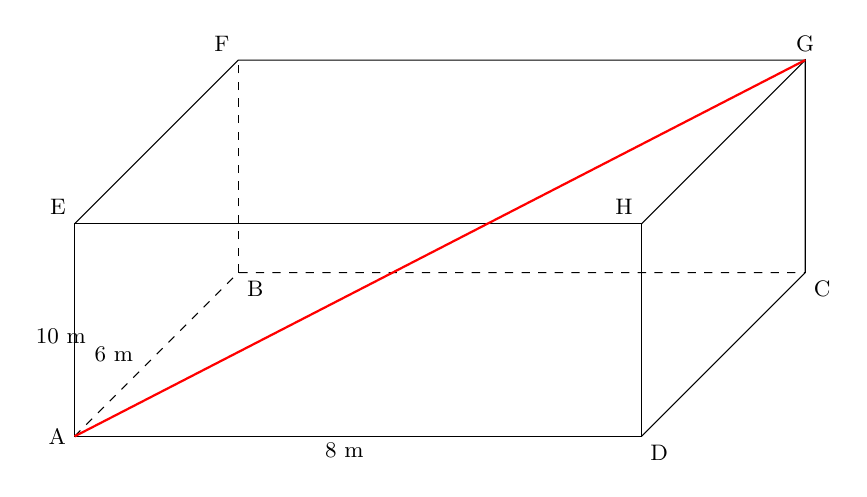
\begin{tikzpicture}[scale=0.9, transform shape]
    % Define the points of the cuboid
    \coordinate (A) at (0,0,0);
    \coordinate (B) at (0,0,-6);
    \coordinate (C) at (8,0,-6);
    \coordinate (D) at (8,0,0);
    \coordinate (E) at (0,3,0);
    \coordinate (F) at (0,3,-6);
    \coordinate (G) at (8,3,-6);
    \coordinate (H) at (8,3,0);

    % Draw the visible edges of the cuboid
    \draw (A) -- (D) -- (H) -- (E) -- cycle; % bottom face
    \draw (D) -- (C) -- (G) -- (H); % right face
    \draw (E) -- (F) -- (G); % top face

    % Draw the hidden edges of the cuboid
    \draw[dashed] (A) -- (B) -- (C);
    \draw[dashed] (B) -- (F);

    % Draw the space diagonal
    \draw[thick, red] (A) -- (G);

    % Place the labels with smaller font size
    \node at (A) [left,font=\small] {A};
    \node at (B) [below right,font=\small] {B};
    \node at (C) [below right,font=\small] {C};
    \node at (D) [below right,font=\small] {D};
    \node at (E) [above left,font=\small] {E};
    \node at (F) [above left,font=\small] {F};
    \node at (G) [above,font=\small] {G};
    \node at (H) [above left, font=\small] {H};

    % Dimension labels
    \node at (4, 0, 0.5) [font=\small] {$8$ m};
    \node at (-0.6, 0, -3) [font=\small] {$6$ m};
    \node at (0, 1.6, 0.5) [font=\small] {$10$ m};
\end{tikzpicture}
\end{center}

\noindent The storage box has the dimensions $AD = 8$ m, $AB = 6$ m and $AE = 10$ m.

\noindent Calculate the length of the diagonal $AG$, which runs from one corner of the box to the diagonally opposite corner.

\vspace{4.5cm}

\begin{flushright}
    \answerunit{m}{3}
\end{flushright}
\end{question}
